\documentclass[sigconf]{acmart}

\settopmatter{printacmref=false} % Removes citation information below abstract
\renewcommand\footnotetextcopyrightpermission[1]{} % removes footnote with conference information in first column
\pagestyle{plain} % removes running headers

\usepackage{booktabs} % For formal tables
% \usepackage[utf8]{inputenc}    
% \usepackage[T1]{fontenc}
\usepackage{graphicx}
% \usepackage{url}
% \usepackage[breaklinks]{hyperref}


\DeclareUnicodeCharacter{00A0}{ }

% Copyright
%\setcopyright{none}
%\setcopyright{acmcopyright}
%\setcopyright{acmlicensed}
\setcopyright{rightsretained}
%\setcopyright{usgov}
%\setcopyright{usgovmixed}
%\setcopyright{cagov}
%\setcopyright{cagovmixed}
\usepackage{graphicx}

% \copyrightyear{2017}


% \acmArticle{4}
% \acmPrice{15.00}


\begin{document}
\title{A Chance to Work}
\subtitle{Understanding the composition of foreign workers 
pursuing \\specialty occupations on the United States H1-B visa
}


\author{\textbf{Alexander Buddenbaum}}
\affiliation{%
  \institution{Georgia Institute of Technology}
%   \streetaddress{North Avenue}
  \city{Shenzhen} 
  \country{China}
}
\email{alex.budd@gatech.edu}

\author{\textbf{Qinrui Li}}
\affiliation{%
  \institution{Georgia Institute of Technology}
%   \streetaddress{North Avenue}
  \city{Shenzhen} 
  \country{China} 
}
\email{qli449@gatech.edu}

\author{\textbf{Tianyu Li}}
\affiliation{%
  \institution{Georgia Institute of Technology}
%   \streetaddress{North Avenue}
  \city{Shenzhen} 
  \country{China}  
}
\email{tli303@gatech.edu}


\author{\textbf{Chuanqi Liu}}
\affiliation{%
  \institution{Georgia Institute of Technology}
%   \streetaddress{North Avenue}
  \city{Shenzhen} 
  \country{China}
}
\email{cliu732@gatech.edu}

\author{\textbf{Tianshu Tao}}
\affiliation{%
  \institution{Georgia Institute of Technology}
%   \streetaddress{North Avenue}
  \city{Shenzhen} 
  \country{China} 
}
\email{ttao35@gatech.edu}



\maketitle
\pagestyle{plain}
\section{Introduction}


The H1-B visa program allows employers in the United States to hire temporary foreign workers specializing in one of many key occupations.  
To date, numerous studies have been conducted on recent years’ certification data in an attempt to analyze hiring trends. 
However, the usefulness of these studies remains to be questioned as they generally lack interactive visualizations for the user to gain 
insight from this information. In this study, we seek to understand recent hiring trends among US employers as well as the makeup of 
applications for these roles to project economic sectors with growth potential, creating meaningful visualizations for potential work 
visa applicants to interpret current data, and predict the outcome of future applications.


\section{Related work}


As annual H1-B application records are publicly available through the US Department of Labor, 
this data has been a popular topic for machine learning researchers as well as online enthusiasts.  
The topic has also inspired several versions of truncated datasets that have been aggregated by several websites as a resource 
for international applicants, and basic analyses appear frequently in academic journals. The general consensus among 
scholarly literature points to an overall positive economic impact by H1-B workers in the United States (Butler 2012, Peri 2014) and 
skilled immigrant workers successfully integrate into the general population (Grimm 2019, Hermansen 2022). 
Interestingly, none of these studies or websites have successfully integrated the database, 
visualizations, and prediction algorithms under one application. 



We have considered several methods for data cleaning and integration. H1-B application data from the US DOL total over 3 million 
records from 2017 to 2021. Chatterjee et al., use Python packages Pandas and Numpy for data cleansing, including the 
completion of incomplete data in H1-B application data, column name renaming and subset selection (Chatterjee 2021). Specific operations can be done 
by calling Python packages. Looking closely at their data, however, we found that not only is it from a non-official and unverifiable 
source; their records are also severely truncated, and did not effectively consolidate job titles with negligible spelling variations. 
Perhaps this truncation and lack of cleansing was out of convenience, but unfortunately this was the case for the majority of studies 
we read during preliminary research. As the datasets among the different years generally only differ by a few column names while 
retaining similar organization, we find it more convenient to use open-sourced applications such as OpenRefine to clean the data, selecting features 
that may be the most meaningful to the reader (Chadha 2021).  
Dombe et al. use SQLite for its lightweight data storage and access (Dombe 2020).  



Several online databases exist providing similar information. The most accurate and comprehensive websites include H1-B Grader and 
One Point Three Acres, which have aggregated US Department of Labor statistics into textual tables which allow for filtering based 
on attributes such as country of origin, job title, sponsoring employer, and salary band(1Point3Acres 2022, H1BGrader 2022). These are relatively complete 
relational database systems with interactive visualizations. The data is also collected directly from the US DOL and up to date. 
As the data provided by US DOL is in XLS format and consists of over 26 attributes in its initial form, the SQL-style database used 
by these websites appears most appropriate. However, these websites are unable to predict application outcomes for users, thus the 
users must perform their own extrapolations based on their subjective interpretations of recent trends.



Most academic studies rely on various Python libraries for visualizations. Tandon et al compares Python and Tableau as accessible technologies 
for quickly producing charts (Tandon 2021). A similar approach is taken by Chavda et al, analyzing records with Apache Hive and Pig with Tableau 
visualizations (Chavda 2019). We elected to use D3 in Javascript for its rich features and greater availability of documentation 
for creating interactive charts. 



The majority of the research to date compares the performance of several machine learning algorithms in predicting application outcomes. 
Random Forest appears to be the most popular model among other studies (Sundararaman 2017), but other methods have been tested as well. 
Swain et al. compared the accuracy of random forest, k-means clustering, and logistic regression algorithms for predicting 
H1-B application acceptance based on roughly 3 million data points from 2011 to 2016 (Swain 2018), and Chatterjee et al. propose an artificial 
neural network (Chatterjee 2021). They also show a variety of static charts, but the charts only compare across one dimension at a time. The data is 
also nearly ten years old. While these studies set us in a good direction for doing some basic analysis, we seek to augment them 
through an interactive visualization allowing the user to view results based on multiple attributes such as salary and location. 
Thakur et al apply seven classification models - Decision tree, C5.0, Random
Forest, Naïve Bayes, Neural Network and SVM - to predict the status of each H1-B application (Thakur 2018). 
Interestingly, their C5.0 decision tree model proved the most accurate on the same data set used by Swain et al in their research. 
Their liberal use of bar charts makes some of their findings hard to follow. Similar results were found by Jethwani et al, who 
achieved the highest prediction accuracy with a decision tree as opposed to random forest and logistic regression (Jethwani 2019). 
We will run a more recent data set to better reflect 
current trends, and instead of comparing several classifiers for their accuracy, we will focus more on providing meaningful insights 
to users through the dynamic integration of the charts.



The method espoused by Raunak Roy uses the collected feedback in applying the analytic hierarchy process and entropy 
weight method to evaluate the data analysis and prediction model (Roy 2021). This method decomposes the decision-making problem into different 
hierarchical structures according to the order of general objectives, sub objectives at all levels, evaluation criteria and specific 
standby choice. Then, the problem is reduced to the determination of the relatively important weight of the lowest level, such as 
schemes and measures for decision-making, relative to the highest level - the overall goal or the arrangement of the relative 
advantages and disadvantages, so as to judge whether the prediction scheme we provide can meet the needs of users on whether to 
apply for H1-B visa.


\section{Proposed method}


In order to show comprehensive aspects of H1-B statistics to potential users, we propose a set of interactive visualizations, 
employing multiple widely used D3.js charts implemented in Vue and Flask.  The data is publicly available, and all the tools 
are open source and can be deployed from a consumer-grade computer. As such, this project requires no special funding. 



We retrieve H1-B application data from years 2017 to 2021 from the US Department of Labor. All records from these five 
years in their original XLS format totaled over 1.5Gb. By accessing data directly from its original source, we can 
guarantee our data will have the highest possible integrity for more accurate evaluation and predictions. 
There are some inconsistencies in the naming and ordering of columns from year to year, as well as the addition of columns that are not pertinent to 
our analysis.  We use OpenRefine to clean and standardize the data, dropping columns that are not pertinent to our 
analysis, thus making the file sizes manageable before consolidating into CSV files aggregated by year. 
\begin{figure}
  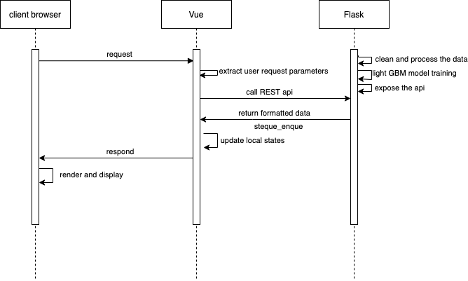
\includegraphics[width=\linewidth]{fig4.png}
  \caption{App Process Flow}
  \label{fig:appprocessflow}
\end{figure}

Users will select the attributes they are interested in on our portal page. Their request will be passed to our 
backend REST API, implemented by Python Flask. The API will then send the corresponding statistics back to the 
front-end interface. The user interface will then process the data and render the chart on the newly-directed page, 
where the user can view and interact with the chart using their cursor. The front-end application, based on Vue and D3.js, 
will have an interactive interface to provide the user rich choices of viewing, comparing, selecting and searching by certain fields. 



As mentioned in Related Work, other implementations exist on the Web. Our implementation is distinct from these earlier 
implementations by including several innovations or improvements. Our system provides users with more selections and 
chart types that are more relevant to the user, such as a US choropleth with state-by-state comparison. 
We provide more relevant details with the ability to combine search parameters such as state and salary. 
We also introduce H1-B application outcome prediction through machine learning methods, a feature we have yet to find on 
any frequently accessed website. A list of innovations and improvements is listed in Appendix B.  


We also construct a model that can predict the probability that a given application will be certified by the DOL. 
As mentioned above, the data requires minimal cleansing and feature engineering, dropping some unimportant features 
by the results of correlation and manual selection. We split the data 70\%-30\% for training and testing. 
We define our task as a binary classification, setting the “Certified” status as 1 and all other non-certified statuses 
as 0 to train our model. For the model, we choose a gradient boosting decision tree model named LightGBM because the data 
is nonlinear as we believe that this tree model shows improved performance over some of the commonly applied linear models. 
We cross-validate the data with 10 folds. 



\begin{figure}
  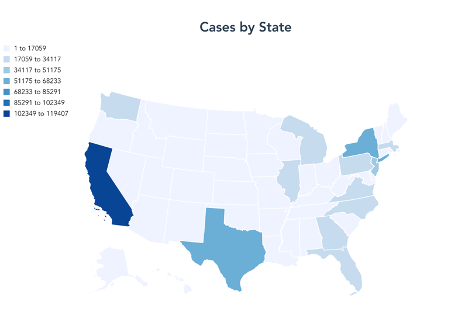
\includegraphics[width=\linewidth]{fig1.png}
  \caption{Choropleth}
  \label{fig:choropleth}
\end{figure}



\section{Experiments and Evaluation}

We have followed the original work distribution, which is distributed evenly among all 5 team members, 
with each member responsible for one component as well as making limited contributions to other components (see Appendix A). 


\subsection{Data Preprocessing and Feature Selection}

The raw data from US Department of Labor, organized by fiscal quarter, 
included as many as 30 attributes depending on the reporting year, 
making the data files quite cumbersome to manage. 
As several of our members are familiar with the H1-B application process, 
we were able to complete an initial manual feature selection with the assistance 
of the official US DOL documentation using OpenRefine, 
removing several attributes clearly irrelevant to our study. 
We retained the following attributes for our analysis:

  \begin{itemize}
    
  \item \textbf{Case number}: Unique identifier for each application record.
  \item \textbf{Case status}: Result of petition, 
  ie. Certified, Withdrawn, Denied. 
  \item \textbf{SOC name}: Official occupation title as defined by US Bureau of Labor Statistics, 
  ie. Software Developer, Computer Systems Analyst.
  \item \textbf{NAICS code}: Primary industry sector/vertical of employer as defined by 
  the North American Industry Classification System, 
  ie. Manufacturing, Information.
  \item \textbf{Full time position}: Whether the position is full-time.
  \item \textbf{Worksite state}: State of primary location of employment,
  ie. CA, NY, TX.
  \item \textbf{Worksite city}: City of primary location of employment, 
  ie. Menlo Park, Austin.
  \item \textbf{Employer name}: Name of petitioning employer,
  ie. Amazon, Deloitte.
  \item \textbf{Employer Business DBA}: Alternate name for employer. 
  \item \textbf{Total workers}: Number of workers included in a single petition. 
  Often the case when an employer hires several workers with the same occupation title. 
  \item \textbf{Wage rate of pay - From}: Minimum prevailing annual salary for the position.
  ie. \$85,000.
  \item \textbf{Wage - unit of pay}: Our analysis concentrates on USD paying occupations.

  \end{itemize}

A test run with the data using several gradient boosted decision tree learners, 
mentioned in more detail below, achieved an F1 score of 98\% on both testing 
and training data; therefore, we retained the exact attributes from our manual selection. 



% EMPLOYER NAME,1513.5
% WORKSITE CITY,490.5
% NAICS CODE,319.9
% SOC NAME,240.4
% WAGE_RATE_OF_PAY_FROM,99.9
% WORKSITE_STATE,88.2
% EMPLOYER_BUSINESS_DBA,82.6
% PREVAILING_WAGE,81.9
% WAGE_UNIT_OF_PAY,32.9
% PW_UNIT_OF_PAY,24.6
% TOTAL_WORKERS,22.2
% FULL_TIME_POSITION,3.4


We apply regular expressions to remove superfluous characters from the records, 
such as commas and dollar signs from some of the wage entries, 
as well as correct input errors and standardize capitalization of Case Status entries, 
and standardized Worksite State to display the full name of their respective states.  


We discovered several outliers with wages that are far beyond the typical range. 
We set an accepted wage ceiling at \$350,000 to mitigate any potential skewing of results 
by these outliers. 


\subsection{Prediction Algorithm}
Based on existing literature, boosted decision tree has generally proven 
the most accurate with historical application data due to its non-linearity. 
We investigated several open-source gradient boosted frameworks, including XGBoost, 
Yandex’s CatBoost, and Microsoft’s LightGBM. We tested all three frameworks on 
all 5 years of data with a 30\%-70\% training split and 10-fold cross validation. 
While all provided very high accuracy and an F1 score of 97\%, our choice of LightGBM ran 20\% faster than the others. 

[figure showing accuracy and speed of different frameworks]


\subsection{Integration}
We integrated all visualizations and our predictor within a single 
web application built on the Flask framework, with a responsive interface using Vue. 
The user clicks a link to one of several visualizations of any given year's applications 
by state, employer, or job title. 

The user may also review application trends by similar criteria using a drop-down list. 
We hoped to include elastic search supporting multiple user-defined parameters, but this 
proved to be too cumbersome for the scope of this project. 

Due to the like-kind nature between objects, we show (XXX) with bar charts, and line charts for (XXX). 


Naturally, the US choropleth map fits best for geographical comparison among states. To incrementally 
provide more information based on user feedback, each state displays a tooltip upon cursor hovering, 
which includes key details such as the total applications for that year, the top employer, and the top 
job title.  


Although the overall volume of our data is quite large at roughly 450 MB, 
each individual record size is trivial after feature selection; thus, we 
were able to handle the processing and querying of these records through Pandas data frames, 
bypassing the need for a database. 


(Include visualizations by year, state, and occupation. ASDFASDFASDFASDFASDFASDFASDFASDFASDFASDF)


We include the multiple criteria filters for the choropleth, line and 
bar charts for single criteria comparisons. 



\subsection{Analysis}

Overall applications ranged from XXX in YYYY, to XXX in YYYY, averaging XXX per year. 
We can see a (spike/drop) in YYYY, followed by a (spike/drop) in YYYY. 
Incidentally, (ABCDEFG) took place in YYYY, which may provide an explanation for (ASDFASDFASDF).


We can see from the US choropleth map that for each of the five years from 2017 to 2021, applications are mostly 
concentrated in the top three states of California, 
New York, and Texas, which incidentally were among the most populous US states during this period. 
Interestingly, Florida, the third most populous state, is not among the top three states for certified applications. 


We found the most influential attribute by far to be the employer sponsoring 
the application. This begs the question: What practices are these employers employing 
to hire the workers that most closely match US strategic interests? 
Is this the result of best-in-class hiring practices, or is it primarily due to 
recent trends and outpaced growth in selected industry verticals? 
Or is there encouragement to stimulate economic growth in certain geographic areas? 


Worksite city came in as a distant second with respect to the employer. 
With regards to location, the difference in significance between worksite city 
and worksite state is staggering, with worksite city showing six times more significance 
than the worksite state. This indicates that states themselves do not have an absolute advantage 
when it comes to application certification. One may argue that states hosting clusters of 
the more successful cities do indeed enjoy such hegemony, but our data is inconclusive in this regard.
Indeed, the metropolitan area of the company plays a much more important role than the state alone. 


As the initial premise for the H1-B program is to bring in qualified workers in specialty occupations with urgent 
talent needs, we expected industry and job title to play a more important role than the above two attributes. Their significance 
score are high; however, they place immediately after employer and worksite city. 


The remaining attributes ranged from having a small to negligible effect on the prediction results. 


.......insert feature importance figure here.....




\begin{figure}
  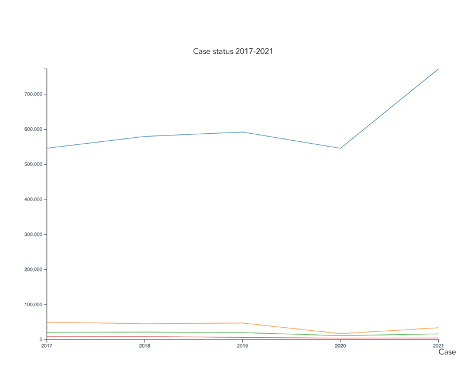
\includegraphics[width=\linewidth]{fig2.png}
  \caption{Line chart}
  \label{fig:linechart}
\end{figure}

\section{Conclusion}

During the first phase of this project, 
we have successfully applied the skills and leveraged the tools touched upon in class to devise a novel solution for a 
real need among international students. In an effort to quickly become proficient in this domain, we have also studied 
the intricacies of the US work visa application process, familiarizing ourselves with the geography and industry makeup 
of the United States. 

We are on schedule to complete our experiment and have a working application by our mid April deadline, at which time we 
look forward to testing its efficacy with a student survey. 


\begin{figure}
  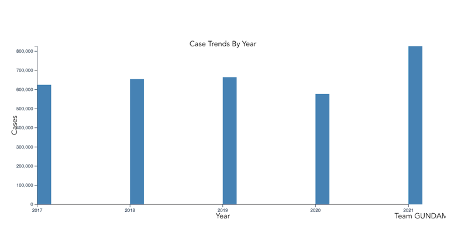
\includegraphics[width=\linewidth]{fig3.png}
  \caption{Bar chart}
  \label{fig:barchart}
\end{figure}


\appendix

\section{Work distribution}

\begin{itemize}
	\item Project coordinator: Tianshu
	\item Data collection, cleansing, standardization, feature selection: Alexander, Tianyu
	\item ML algorithm design: Chuanqi 
	\item UI and visualization design, frontend implementation: Tianshu
	\item Database design, backend implementation: Tianyu
	\item Documentation: Alexander, Qinrui, Chuanqi, Tianshu, Tianyu
	
\end{itemize}

All team members have contributed similar amount of effort and results to this project.

\section{Innovations}
\begin{itemize}
	\item More selections and chart types that are more relevant to the user, such as a US choropleth with state-by-state comparison
	\item Ability to combine search parameters such as state and salary
	\item Interactive H1-B application outcome prediction through machine learning

\end{itemize}



\begin{thebibliography}{12}

\bibitem{}

\textit{}
Peri, G., Shih, K. Y., \& Sparber, C. 
(2014). 
Foreign STEM workers and native wages and employment in US cities (No. w20093). 
\textit{National Bureau of Economic Research. }
\url{https://www.nber.org/system/files/working_papers/w20093/w20093.pdf}.

\bibitem{}
Butler, E. W. 
(2012). 
The H-1B visa immigration program: Analysis and comments. 
\textit{International Journal of Business and Social Science, 3(9).}
\url{https://citeseerx.ist.psu.edu/viewdoc/download?doi=10.1.1.1066.7924&rep=rep1&type=pdf}.


\bibitem{}
Hermansen, A. S. 
(2022). 
Visualizing Intergenerational Immigrant Assimilation at Work. 
\textit{Socius,} 8, 23780231211072590.
\url{https://journals.sagepub.com/doi/full/10.1177/23780231211072590}.

\bibitem{}
Grimm, A. 
(2019). 
Studying to stay: Understanding graduate visa policy content and context in the United States and Australia. 
\textit{International Migration,} 57(5), 235-251. 
\url{https://ieeexplore.ieee.org/stamp/stamp.jsp?tp=&arnumber=9664747}.

\bibitem{} 
	H-1B Program. 
\textit{United States Department of Labor.} 
(2022). 
Retrieved 1 April 2022. 
\url{https://www.dol.gov/agencies/whd/immigration/h1b}.

\bibitem{}
Chatterjee, P., Velpuru, M. S., \& Jagadeeswari, T. 
(2021). 
Success of H1-B VISA Using ANN. 
\textit{In Machine Learning and Information Processing (pp. 491-499).}
 Springer, Singapore.

\bibitem{}
Thakur, P., Singh, M., Singh, H., \& Rana, P. S. 
(2018). 
An allotment of H1B work VISA in USA using machine learning. 
\textit{International Journal of Engineering \& Technology, 7(2.27), 93-103. }
\url{https://www.researchgate.net/profile/Prashant-Rana-4/publication/328488339_An_allotment_of_H1B_work_visa_in_USA_using_machine_learning}.

\bibitem{}
Dombe, A., Rewale, R., \& Swain, D. 
(2020). 
A deep learning-based approach for predicting the outcome of H-1B VISA application. 
\textit{In Machine Learning and Information Processing (pp. 193-202).}
 Springer, Singapore.

\bibitem{}
Visa Tracker - 1Point3Acres. 
(2022). 
Retrieved 1 April 2022.  
\\\url{https://visa.1point3acres.com/}.

\bibitem{}
H1B Database 2022 - Sponsors, Salaries, Approvals, Grades!. 
(2022). 
Retrieved 1 April 2022. 
\\\url{https://h1bgrader.com/}.

\bibitem{}
Tandon, A. 
(2021). 
ANALYSIS OF IMMIGRATION TRENDS IN THE US TO DISCOVER PATTERNS AND MAKE BETTER POLICY DECISIONS.
\\\url{https://scholarworks.lib.csusb.edu/cgi/viewcontent.cgi?article=2387}.

\bibitem{}
Tableau.
Retrieved 1 April 2022.
\\\url{https://tableau.com}.

\bibitem{}
CHAVDA, J. 
(2019). 
Big Data analysis on H-1B Visa Application in the United States.
\url{https://www.researchgate.net/profile/Jyoti-Chavda/publication/341132236_Big_Data_analysis_on_H-1B_Visa_Application_in_the_United_State/}.

\bibitem{}
Sundararaman, D., Pal, N., \& Misraa, A. K. 
(2017). 
An analysis of nonimmigrant work VISAs in the USA using machine learning. 
\textit{Int. J. Comput. Sci. Secur.(IJCSS), 6.}
\url{https://dhanasekar-s.github.io/research/3paper.pdf}.

\bibitem{}
Swain, D., Chakraborty, K., Dombe, A., Ashture, A., \& Valakunde, N. 
(2018, December). 
Prediction of H1B Visa Using Machine Learning Algorithms. 
\textit{In 2018 International Conference on Advanced Computation and Telecommunication (ICACAT) (pp. 1-7).} 
IEEE. 

\bibitem{}
Jethwani, G., Sachdeva, A., \& Goswami, M. 
(2019). 
An Empirical Analysis of ML Algorithms. 
\textit{Proceedings of International Conference on Sustainable Computing in Science, Technology and Management (SUSCOM),} 
Amity University Rajasthan, Jaipur-India.

\bibitem{}
Chadha, A. S., \& Shitole, A. 
(2021, November). 
A Hybrid Machine Learning Model Approach to H-1B Visa. 
\textit{2021 3rd International Conference on Electrical, Control and Instrumentation Engineering (ICECIE)} (pp. 1-8). 
IEEE.
\url{https://www.researchgate.net/publication/357663888_A_Hybrid_Machine_Learning_Model_Approach_to_H-1B_Visa}.

\bibitem{}
Roy, R. (2021). 
Data Analysis of H1B Visa Applications.

\bibitem{}
D3: Data Driven Documents. 
Retrieved 1 April 2022. 
\\\textit{https://d3js.org/.}

\bibitem{}
Vue. 
Retrieved 1 April 2022. 
\\\textit{https://vuejs.org/.}

\bibitem{}
Flask. 
Retrieved 1 April 2022. 
\\\textit{https://flask.palletsprojects.com/en/2.1.x/.}

\bibitem{}
OpenRefine. 
Retrieved 1 April 2022. 
\\textit{https://openrefine.org/.}

\bibitem{}
LightGBM. 
\textit{Microsoft.} 
Retrieved 1 April 2022. 
\\\textit{https://github.com/microsoft/LightGBM.}




\end{thebibliography}

\end{document}
